\documentclass{article}
\usepackage[utf8]{inputenc}
\usepackage{enumitem}
\usepackage{graphicx}
\usepackage{listings}
\usepackage{amssymb}
\usepackage{hyperref}
\graphicspath{{./notepics/}}
\hypersetup{colorlinks=true, urlcolor=blue}
% swnat = start w/ name and today
\newcommand{\swnat}[1]{\begin{document} \begin{flushleft} Date of notes: \today \\ #1 \\}
\newcommand{\iit}{\item}
\newcommand{\iitsub}[1]{\begin{itemize} \item{#1} \end{itemize}}
\newcommand{\mathline}[1]{\vspace*{0.75em}\centerline{#1}}
\newcommand{\fancyL}{$\mathcal{L}$}
\newcommand{\fancydeltaL}{$\nabla \mathcal{L}$}
\newcommand{\fancyR}{$\mathbb{R}$}
\newcommand{\la}{$\leftarrow$ }
\newcommand{\ra}{$\rightarrow$ }
\newcommand{\setin}{$\in$ }
\newcommand{\firstitemstart}[1]{\section*{#1 Notes} \begin{itemize}[leftmargin=*] \setlength\itemsep{.005em}}
\newcommand{\restitemstart}[1]{\end{itemize} \section*{#1 Notes} \begin{itemize}[leftmargin=*] \setlength\itemsep{.005em}}
% note: can't make a newcommand w/ 'end' 
\newcommand{\docitemend}{\end{itemize} \end{flushleft} \end{document}}
\swnat{CAP 4600 All Notes}
\firstitemstart{1.a. Slide}
\iit In terms of being a superset, AI \ra Machine learning \ra Deep learning.
\iit Symbolic AI (also called GOFAI): term for collection of all methods in AI based in symbolic representation.
\iit Diagram of above: input \& rules \ra [machine] \ra output.
\iit ML programs adjust themselves in response to data they're exposed to.
\iit ML is dynamic and doesn't require human intervention to make certain changes.
\iit Diagram of ML: input \& output \ra [machine] \ra rules.
\restitemstart{1.b. Slide}
\iit ML has paradigms, mostly either through supervised or unsupervised learning.
\iit Supervised learning: ML where model is provided w/ labeled training data.
\iit Features and their corresponding labels are fed into an algorithm in the training process.
\iit The algorithm gradually determines the relationship btw. features and corresponding labels, called a model.
\iit Finding patterns btw. data and labels in supervised ML learning can be expressed mathematically as functions.
\iit Unsupervised learning: identifying meaningful patterns in data (and using that to understand the importance of new data).
\iit Reinforcment learning: at time step $t$, the agent is in state $s_t$, takes action $a_t$, receives reward 
$r_t$, and transitions into state $s_{t+1}$.
\iit Agent has to learn which actions to take at the current state for the maximum rewards.
\iit You also need to provide a way for the agent to interact w/ the game to produce data, physically or virtually.
\restitemstart{2.a. Slide}
\iit Supervised ML learning terminology:
\iit Label: what we seek to predict.
\iit Feature $x_j$: input variable that is used to predict the label, where $j \in \{1,\ldots, n\}$ where $n$ is the number of features.
\iit Many features can be used for projects requesting more regulation.
\iit Example: particular instance of data fed into models
\iit Labeled ex.: includes both features and the label, like: \{features, label\}: (x,y)
\iitsub{Used to train model.}
\iit Unlabeled ex.: only features, like: \{features, ?\}: (x,?)
\iitsub{We use the model once it's done training w/ labeled examples to predict the label on unlabeled examples.}
\iit Training: creating or learning the model.
\iitsub{Show the model $(x,y)$ such that it can learn the relationships btw. feature $x$ and 
label $y$ such that prediction $\hat{y}$ is sufficiently close to the label $y$.}
\iit Inference: means applying the trained model to unlabeled examples (making useful predictions $\hat{y}$)
\iit Regression model: predicts continuous vals. (numerical)
\iit Classification model: predicts discrete vals. (descriptive)
\restitemstart{2.b. Slide}
\iit Linear regression: finding the relationship of data through the formula $y=mx+b$
\iit ML equation is slightly different w/ $\hat{y}=b+w_1 x_1$, where:
\iitsub{$\hat{y}$: predictied label (desired output), $b$ is the bias (y-int.) [also called $w_o$], 
$w_1$ is the weight of feature 1 [weight is similar to slope $m$], and $x_1$ is a feature (known input).}
\iit To infer (predict) $\hat{y}$ for a new val. $x_1$, just substitute $x_1$ val. into this model.
\iitsub{Bigger models would rely on multiple features $x_1, x_2, \ldots, x_n$, each having seperete weights $w_1, w_2, \ldots, w_n$.
\iitsub{For example: a model w/ three features might look like: 
$\hat{y}=b+w_1 x_1+w_2 x_2+w_3 x_3 = b + \sum^{3}_{j=1} w_j x_j$. }}
\restitemstart{2.c. Slide}
\iit Training: examining the examples and adjusting the weights \& bias so that the loss is minimized.
\iit Loss: penalty for a bad prediction, quantifying how bad the model's prediction was on a single example.
\iit The goal of training: finding a set of weights \& biases that have low loss across 
all examples on average (process called empirical risk minimization).
\iit Use of a square loss employed as a loss function (also known as a $L_2$ loss).
\iitsub{If we let $w = (b, w_1, \ldots, w_n)$ be the params. of the model (weights and bias), 
and features be w/ $x = (x_1, \ldots, x_n)$ label $y$, the model will predict $\hat{y} = f_w(x) = b + \sum^{n}_{j=1} w_j x_j. $
\iitsub{The squared loss for a single example the difference btw. label (obs.) $y$ and prediction $\hat{y}$: $(y-\hat{y})^2$.}}
\iit Mean square error (MSE): average squared loss per example over whole dataset:
$MSE(w) = 1/m \sum^{m}_{i=1} (y^{(i)} - \hat{y}^{(i)})^2$.
\iitsub{$m$ is the number of examples, $x^{(i)} = (x_1^{(i)}, \ldots, x_n^{(i)})$ \& $y^{(i)}$ are the features 
and the label of the $i$th example, and $\hat{y}^{(i)}$ is the prediction of the model.
\iitsub{Formally, $\hat{y} = f_w(x^{(i)}) = b + \sum^{n}_{j=1} w_j x_j^{(i)}. $}
Although MSE is heavily used in ML, it isn't the best loss function or the the only practical loss function for every circumstance.}
\restitemstart{2.d. Slide}
\iit Iterative learning: try to reduce loss iteratively (guess a val. of $w_1$ and wait for the system to tell us what the loss is)
\iit If we adapt the weights correctly, we will be decreasing the loss over time. 
The challenge is to find the best possible model as efficiently as possible.
\iitsub{The iterative trial-and-error process that ML algos. use to train a model includes: \\
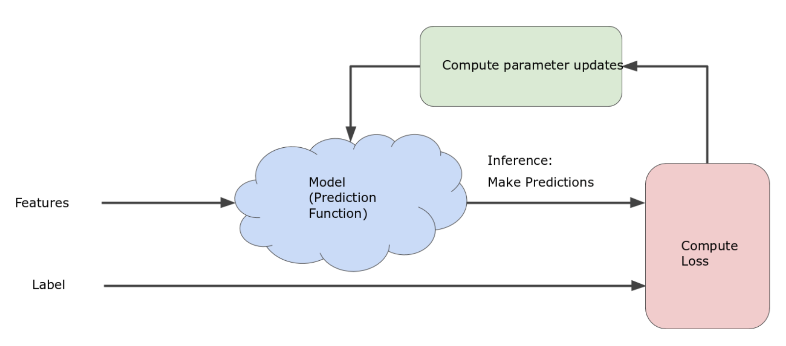
\includegraphics[scale=0.5]{iterative} \centering}
\iit Iterative strats. are prevalent in ML because they scale so well to large data sets. The model takes features $x_1, \ldots, x_n$
as input and returns one prediction $\hat{y}$ as output. 
\iitsub{ If we consider that the simplest lin. reg. model that takes only one feature as input: $\hat{y} = b + w_1 x_1$. 
For lin. reg. problems, we can pick random vals. for the starting positions $b$ \& $w_1$. }
% note: double qoutes must look like {``} for the first part and {''} for the last part
\iit If we look inside the ``Compute parameter updates'' part of the diagram, we can see the ML system examines the val. of the loss function
\& generates new vals. for $b$ \& $w_1$. We can say for now that it devises new vals. \& then the ML system re-evaluates all those features
against all those labels, yielding a new val. for the loss function, which yields new param. values. The learning continues iterating until the ML system discovers the model params. w/ the lowest possible loss. Usually, we iterate until the loss stops changing or at least there are extremely slow changes to the model. If this happenes, we can say the model has converged.
\iit A ML model is trained by starting w/ an init. guess for the weights \& bias and iteratively adjusting those guesses until finding
the weights \& the bias w/ the lowest possible (or sufficiently low) loss are found.
\restitemstart{2.e. Slide}
\iit Gradient descent algo.: When we consider the linear regression model $\hat{y}=f_w(x) = b+w_1 x_1+w_2 x_2+ \ldots + w_n x_n$,
where $w=(w_0, w_1, \ldots, w_n)$, The loss function (MSE): \\ 
\centerline{\fancyL$ $ : \fancyR $^{n+1}$ \ra \fancyR} 
depends on the params. $n+1$ params. $b, w_1, \ldots, w_n$. The loss is given by: \\
\mathline{\fancyL$ $ = $1/m \sum^{m}_{i=1} 1/2(\hat{y}^{(i)} - y^{(i)})^2$}
\mathline{$= 1/m \sum^{m}_{i=1} 1/2(f_w(x^{(i)}-y^{(i)}))^2$}
\mathline{$= 1/m \sum^{m}_{i=1} 1/2(\sum^{n}_{j=1} w_j x_j + b - y^{(i)})^2.$}
\vspace*{-0.125em}\iit For $n=1$, the loss function \fancyL$ $ depends on two params., the bias term $b = w_0$ and the weight $w_1$, \& defines a surface in 3D. For $n > 1$, the loss function \fancyL$ $ cannot be visualized easily. To simplify the plots, we assume that $n = 1$ and the bias term $b = w_0$ is fixed to be 0. Then the loss function \fancyL$ $ depends only on $w_1$ and defines a curve. 
\iit The resulting plot of the loss function \fancyL$ $ is convex (assuming graph is loss over value of weight $w_1$). Even in the general case, the loss function \fancyL$ $ is convex. This is important since problems only have one min. 
Calculating the loss function for all param. values $w_0, \ldots, w_n$ \setin \fancyR $^{n+1}$ would be an inefficient way of finding the min.
Let's examine a better mechanism (very pop. in ML) called gradient descent.
\iit The starting point doesn't matter in the first stage in gradient descent, so we can set $w_i = 0$ or a rand. val.
\iit The gradient descent algo. then calculates the gradient of the loss function \fancyL$ $ at the starting point. The gradient 
\fancydeltaL\setin\fancyR$^{n+1}$ is a vector whose entries $($\fancydeltaL$)_i$ are given by the partial derivs. $\partial$\fancyL$/ \partial w_i$
of the loss function \fancyL$ $ with respect to the weights $w_i$.
\iit The \fancydeltaL$ $ gradient has both a dir. and a mag. 
The graident points which way is closer or farther from the intended target.
The gradient always points in the dir. of steepest increase in the loss function. For the case $n=1$ \& the bias $w_0 = b$ is fixed to be 0, the gradient of the loss function \fancyL $ $ is simply the slope of the curve \fancyL$ $, that is, the deriv. w/ respect to $w_1$. 
\iitsub{The gradient descent algo. takes a step in the direction of the negative gradient $-$\fancydeltaL$ $ to reduce the loss. 
More precisely, the gradient descent algo. updates the starting point as follows: w \la w $- \alpha$\fancydeltaL, where $\alpha$ is the learning rate.}
\iit The gradient vector also has both a dir. \& a mag. The gradient descent algo. multiplies the grad. by a scalar known as the learning rate
(also sometimes called step size) to determine the next point. The learning rate is a so-called hyperparameter: a parameter that is external
to the model.
\iitsub{If the learning rate is too small, learning will take too long, but if it is too large, the next point will perpetually bounce haphazardly
across the bottom of the well. There must be a Goldilocks learning rate for every linear reg. problem.}
\restitemstart{2.f. Slide}
\iit In a gradient descent, a batch is the total number of examples you use to calculate the gradient in a single interation. If a batch encompasses a large data sets (with a huge number of examples and a huge number of features), then the batch could be enormous and take a very long time to compute a single iteration. 
\iit Data redundancy could be useful in data to smoothen out noisy gradients, but enormous batches could have larger amounts of redundancy, increasing computation time.
\iit To counter this, if we choose examples at random from our data set, we could estimate a big average from a much smaller one. 
\iit Stochastic gradient descent (SGD) uses only a single example (batch size of 1) per iteration. Through many iterations, SGD works but is very noisy. ``Stochastic'' refers that the one example comprising each batch is chosen at random.
\iit Mini batch SGD is a compormise b/tw full batch iteration and SGD. A mini-batch is typically b/tw 10 and 1000 examples, chosen at random. It reduces the amount of noise in SGD but is still more efficient than full-batch.
\restitemstart{3. Slide}
\iit Keras is a deep-learning framework for Python that provides a convenient way to define and train alomst any kind of deep-learning model. The Keras documentation is listed as \href{https://keras.io/}{https://keras.io/.} It has the following features:
\iitsub{It allows for the same code to run seamlessly on CPU or GPU. It has a user-friendly API that makes it easy to quickly prototype deep-learning models. It has built-in support for convolutional networks (for computer vision), recurrent networks (for sequence processing), and for any combination of both. It also supports arbitrary network architectures such as multi-input or multi-output models, and layer sharing. It is appropriate for building essentially any deep learning model, from a generative adversarial network to a neural Turing machine.}
\iit Keras is a model-level library, providing high-level building blocks for developing deep-learning models. It doesn't handle low-level operations such as tensor manipulation and differentiation; instead it relies on a specialized, well-optimized library to so, serving as a backend of Keras. Rather, than choosing a single tensor library and tying the implementation of Keras to that library, Keras handles the problem in a modular way. Links to resources used: 
\href{https://www.tensorflow.org/}{TensorFlow},
\href{http://www.deeplearning.net/software/theano/}{Theano},
\href{https://www.microsoft.com/en-us/cognitive-toolkit/}{CNTK},
\href{https://developer.nvidia.com/about-cuda}{CUDA},
\href{https://developer.nvidia.com/cudnn}{cuDNN},
\href{http://www.netlib.org/blas/}{Blas}, \&
\href{http://eigen.tuxfamily.org/index.php?title=Main_Page}{Eigen}.
\iit The typical Keras workflow looks like this:
\iitsub{Define your training data: input tensors and target tensors. Define a network of layers (or model) that maps your inputs to your targets. Configure the learning process by choosing a loss function, an optimizer, and some metrics to monitor. Iterate on your training data by calling the \texttt{fit()} function method of your model.}
\iit TensorFlow is a computational framework for building machine learning models. TensorFlow provides a variety of different toolkits that allow you to construct models at your preferred level of abstraction. You can use lower-level APIs to build models by defining a series of mathematical operations. Alternatively, you can use higher-level APIs (like \texttt{tf.estimator}) to specify predefined architectures, such as linear regressors or neural networks.
\iit The following table summarizes the purposes of the different layers:
\begin{tabular}{|l|l|}
    \hline
    Toolkit(s) & Description \\ \hline \hline
    Estimator \texttt{tf.estimator} & High-level, OOP API \\ \hline
    \texttt{tf.layers/tf.losses/} & Libraries for common model \\
    \texttt{tf.metrics}           & components \\ \hline
    TensorFlow & Lower-level APIs \\ \hline
\end{tabular}
\iit TensorFlow consists of the following two components: a graph protocol buffer used to specify the  computation as a distributed graph \& a runtime that executes the distributed graph. These two components are analogous to Python code and the Python interpreter. The Python interpreter is implemented on multiple hardware platforms to run Python code. Analogously, TensorFlow is implemented on multiple hardware platforms, including CPU, GPU, and TPU (Tensor Processing Unit), to run the graph.
\iit In TensorFlow, the computation is specified as a distributed graph. Nodes in the graph represent operations. Edges are directed and represent passing the result of an operation (a tensor) as an operand to another operation. Tensors are the primary data structure in TensorFlow programs. They are $N$-dimensional (where $N$ could be very large) data structures, most commonly scalars, vectors, or matrices. TensorBoard is used to visualize a computational graph.
\iit Which API(s) should you use? You should use the highest level of abstraction that solves the problem. The higher levels of abstraction are easier to use, but are also (by design) less flexible. We recommend you start with the highest-level API first and get everything working. If you need additional flexibility for some special modeling concerns, move one level lower. Note that each level is built using the APIs in lower levels, so dropping down the hierarchy should be reasonably straightforward.
\restitemstart{4. Slide}
\iit The fundamental data structure in neural networks is the layer. A layer is a data-processing module that takes as input one or more tensors and that outputs one or more tensors. Some layers are stateless, but more frequently layers have a state: the layers weights, one or several tensors learned with stochastic gradient descent, which together contain the network's knowledge.
\iit Different layers are appropriate for different tensor formats and different types of data processing.
\iit Simple vector data, stored in 2D tensors of shape \texttt{(samples, features)} is often processed by densely connected layers, also called fully connected layers (the \texttt{Dense} class in Keras). Sequence data, stored in 3D tensors of shape \texttt{(samples, timesteps, features)}, is typically processed by recurrent layers such as long-short term memory (LSTM) layer. Image data, stored in 4D tensors, is usually processed by 2D convolutional layers (\texttt{Con2D}). \href{https://keras.io/layers/core/}{Core}, \href{https://keras.io/layers/convolutional/}{Convolutional}, \& \href{https://keras.io/layers/recurrent/}{Recurrent} layer descriptions here.
\iit You can think of layers as LEGO bricks of deep learning. Building deep-learning models in Keras is done by combining compatible layers to form useful data-processing pipelines. Layer compatibility means that every layer will only accept input tensors of a certain shape and will return output tensors of a certain shape. When using Keras, you don't have to worry about compatibility, because the layers you add to your model are dynamically built to match the shape of the incoming layer.
\lstset{language=Python,basicstyle={\small\ttfamily}}
\begin{lstlisting}
from keras import models
from keras import layers

network = models.Sequential()

network.add(layers.Dense(512,
                         activation='relu',
                         input_shape=(28 * 28,)))

# no need to specify input_shape for second layer
network.add(layers.Dense(10,
                         activation='softmax')) 
\end{lstlisting}
\iit The second layer didn't receive an input shape argument -- instead, it automatically inferred its input shape as being the output shape of the first layer.
\iit A deep-learning model is a directed, acyclic graph of layers. The most common topology is a linear stack of layers, mapping a single input to a single output. These can be implemented using \texttt{models.Sequential()}. Initially, we will only work with linear stacks of layers. Later, we will also look at other network topologies such as two-branch networks, multi-head networks, and inception blocks.
\iit The topology of a network defines a hypothesis space. By choosing a network topology, you constrain your space of possibilities (hypothesis space) to a specific series of tensor operations, mapping input data to output data. You'll be then searching for a good set of values for the weight tensor involved in these tensor operations using stochastic a variant of gradient descent. Picking the right network architecture is more art than a science. We will study explicit principles for building neural networks and develop intuition as to what works or doesn't for specific problems.
\iit Once the network architecture is defined, you still need to do two things: \href{https://keras.io/losses/}{Loss function (objective function)}: The quantity that will be minimized during training. It represents a measure of success for that task at hand. \href{https://keras.io/optimizers/}{Optimizer}: Determines how the network will be updated based on the loss function. Implements a specific variant of stochastic gradient descent (SGD).
\iit Choosing the right objective function for the right problem is extremely important: your network will take any shortcut it can, to minimize the loss. Fortunately, there are simple guidelines you can use to choose the correct loss for common problems such as classification, regression, and sequence prediction.
\begin{tabular}{|c|c|c|}
\hline
Problem type & Last-layer activation & Loss function \\ \hline\hline
Binary classification & \texttt{sigmoid} & \texttt{binary\_crossentropy} \\ \hline
Multiclass,  & \texttt{softmax} & \texttt{categorical\_crossentropy} \\
single-label classification & & \\ \hline
Multiclass,  & \texttt{sigmoid} & \texttt{binary\_crossentropy} \\
multi-label classification & & \\ \hline
Regression & \texttt{None} & \texttt{mse} \\
to arbitrary values & & \\ \hline
Regression & \texttt{sigmoid} & \texttt{mse} or \\
to values in $[0,1]$ & & \texttt{binary\_crossentropy} \\ \hline
\end{tabular}
\restitemstart{5. Slide}
\iit To gain some intuition about generalization, let's look at the following three figures. Assume that each dot in these figures represents a tree's position in a forest. The two colors have the following meanings: The blue dots represent sick trees \& the orange dots represent healthy trees. Can you imagine a good model for predicting subsequent sick or healthy trees? 
\iit Look now at the next figure, which shows how a certain machine learning model separated the sick trees from the healthy trees. Note that this model produced a very low loss. At first glance, this model appears to do an excellent job of separating the healthy trees from the sick ones. Or does it? The next figure shows what happened when we added new data to the model. It turned out that the model adapted very poorly to the new data. Notice that the model miscategorized much of the new data. 
\iit The model shown did a bad job predicting new data. The model overfits the peculiarities of the training data. An overfit model has a low loss on the training data, but it has a high loss of the test data (new unseen data). Overfitting is caused by making a model more complex than necessary. The fundamental tension of machine learning is between fitting our training data well, but also fitting it as simply as possible.
\iit Machine learning's goal is to predict well on new data drawn from a (hidden) true probability distribution. Unfortunately, the model can't see the whole truth; the model can only sample from a training data set. If a model fits the current examples well, how can you trust the model will also make good predictions on never-before-seen examples?
\iit 

\restitemstart{\href{https://colab.research.google.com/drive/1CdwvzRhFNIlhp1mWVWFXSXAsmRFWvASq}{Python3}}
\iit Primitive Datatypes -- straighforward
\iit Control Statements (if, for, while, etc.) -- remember to add ``:'' after statements and to indent
\restitemstart{\href{https://colab.research.google.com/drive/1eECClMU1r-Y9hzPnRw89__jC3nw3C-zD}{Effect of Learning Rate on Gradient Descent for Finding Minima of Univariate Functions}}
\iit Notebook for experimenting with different learning rates and understanding what could go wrong when applying gradient descent with a poorly chosen learning rate.
\iit Overstepping in the learning rate could have massive consequences, while also getting stuck in a local minimum could stall the progress of the ML process.
\docitemend
